\documentclass[main]{subfiles}
\begin{document}

%@@@@@@@@@@@@@@@@@@@@@@@@@@@@@@
% summarizes lecture 11
% author: 

\section{Silicon Neurons}
\subsection{What is a neuron and what are its components?}
The basic anatomical unit in the nervous system is specialised cell called the neuron.

\cite{book:Mead}

\begin{enumerate}
\item Synapse
\item Soma
\item Dendrite
\end{enumerate}
\subsection{What types of models are used to simulate neurons?}
\subsection{How does the spikegeneratng mechanism work?}
\subsection{What is an FI curve?}
\subsection{Can you draw the circuit schematic of the axon-hillock neuron?}
The schematic of the axon-hillock neuron can vary upon the chosen amplification. General schematic is depicted on the figure \ref{fig:neuron_hillock_general}.

\begin{figure}[htbp]
  \centering
  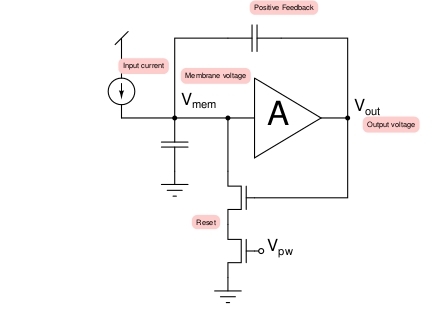
\includegraphics[scale=0.8]{pics/neuron_hillock_general.jpg}
  \caption{The Axon-Hillock circuit \cite{lec11}.}
  \label{fig:neuron_hillock_general}
\end{figure} 

The specific amplification was chosen and is depicted on the Axon-hillock integrate and fire circuit (see fig. \ref{fig:neuron_hillock}).

\begin{figure}[htbp]
  \centering
  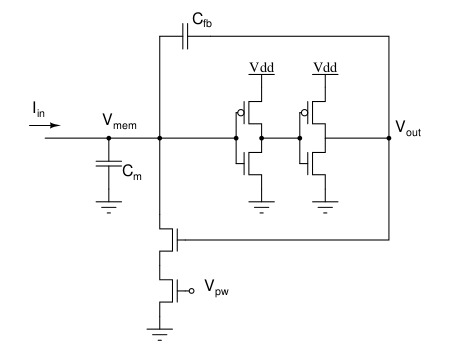
\includegraphics[scale=0.8]{pics/neuron_hillock.jpg}
  \caption{Axon-hillock integrate and fire circuit \cite{lab11}.}
  \label{fig:neuron_hillock}
\end{figure} 


\cite{lab11}.
\todo[inline]{Complete "Silicon Neurons" chapter}
\end{document}